%\documentclass[handout,xcolor=svgnames]{beamer}
\documentclass[xcolor=svgnames]{beamer}
\usepackage[utf8]{inputenc}
\usepackage[english]{babel}
\usepackage{transparent}
\usepackage{booktabs}
\usepackage{xcolor}
\usepackage{numprint}
\usepackage{multicol}


\makeatletter
\newbox\@backgroundblock
\newenvironment{backgroundblock}[2]{%
  \global\setbox\@backgroundblock=\vbox\bgroup%
    \unvbox\@backgroundblock%
    \vbox to0pt\bgroup\vskip#2\hbox to0pt\bgroup\hskip#1\relax%
}{\egroup\egroup\egroup}
\addtobeamertemplate{background}{\box\@backgroundblock}{}
\makeatother

\usetheme{ProsoLight}

\title[Similarity measures]{Measuring Similarity of Educational Items Using Data on Learners' Performance}
\author{\textbf{Ji\v{r}í \v{R}ihák}, Radek Pelánek}
\institute{Masaryk University Brno}
\date{}

\begin{document}
% --------------------------- SLIDE --------------------------------------------
\frame[plain]{\titlepage}
% ------------------------------------------------------------------------------
% --------------------------- SLIDE --------------------------------------------
\begin{frame}
    \frametitle{Adaptive learning}

    \Large

    Adaptive practice systems
    \begin{itemize}
        \item \textbf{items} --- simple questions
        \item practice --- rapid sequence of items
    \end{itemize}


    \vfill
    \centering

    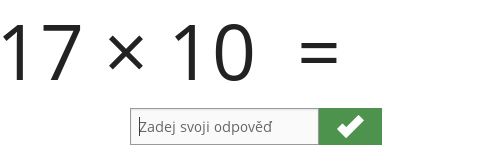
\includegraphics[width=.45\linewidth]{figures/matmat.png}
    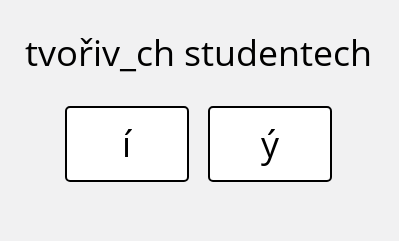
\includegraphics[width=.45\linewidth]{figures/cestina.png}


\end{frame}
% ------------------------------------------------------------------------------
% --------------------------- SLIDE --------------------------------------------
\begin{frame}
    \frametitle{Motivation }
    \Large

    \begin{backgroundblock}{10mm}{30mm}
        \hspace{0.4\linewidth}
        \only<2>{\hspace{0.1\linewidth}}
        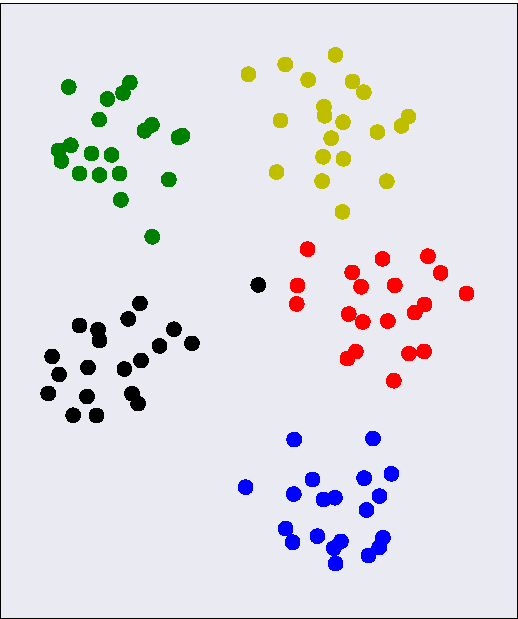
\includegraphics[width=0.4\linewidth]{figures/clustering}<2>
        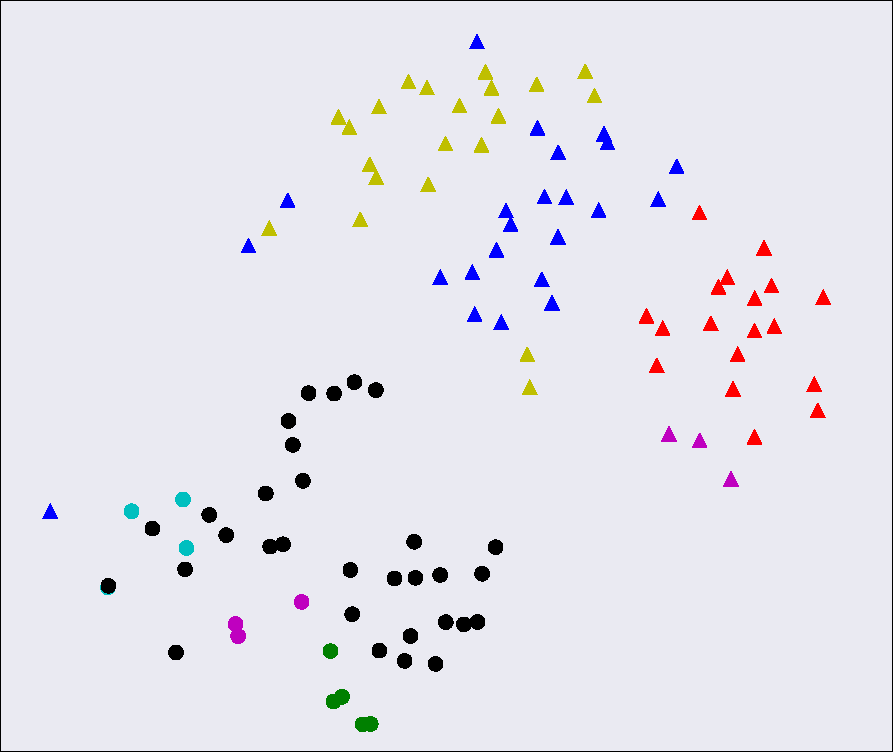
\includegraphics[width=0.6\linewidth]{figures/tsne-cz}<3>
        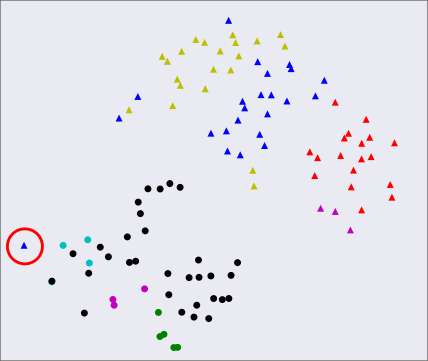
\includegraphics[width=0.6\linewidth]{figures/tsne-cz-outlier}<4>
    \end{backgroundblock}

    Large pool of items
    \large

    \only<1>{
    \begin{itemize}
        \item How to organize these items?
        \item What knowledge components should be use?
        \item Are there some anomalies?
        \item \dots
    \end{itemize}
    }

    \only<2-4>{
    \begin{itemize}
        \item \textbf<2>{clustering}
        \item \textbf<3>{visualization}
        \item \textbf<4>{outlier detection}
        \item \dots
    \end{itemize}
    }

\end{frame}
% ------------------------------------------------------------------------------
% --------------------------- SLIDE --------------------------------------------
\begin{frame}
    \frametitle{General approach}
    \centering
    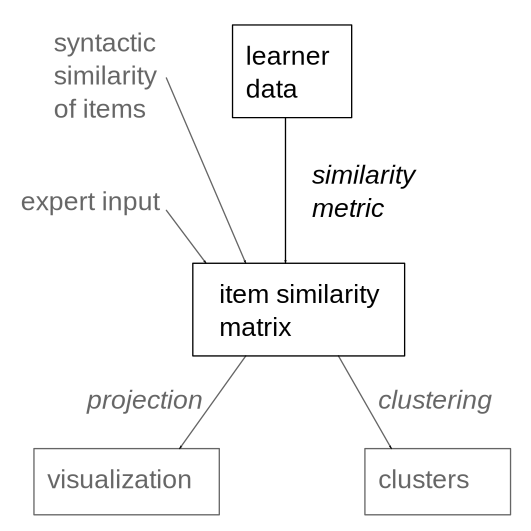
\includegraphics[width=.9\linewidth]{figures/general-approach}
\end{frame}
% ------------------------------------------------------------------------------
% --------------------------- SLIDE --------------------------------------------
\begin{frame}
    \frametitle{Similarity measures}
    \centering
    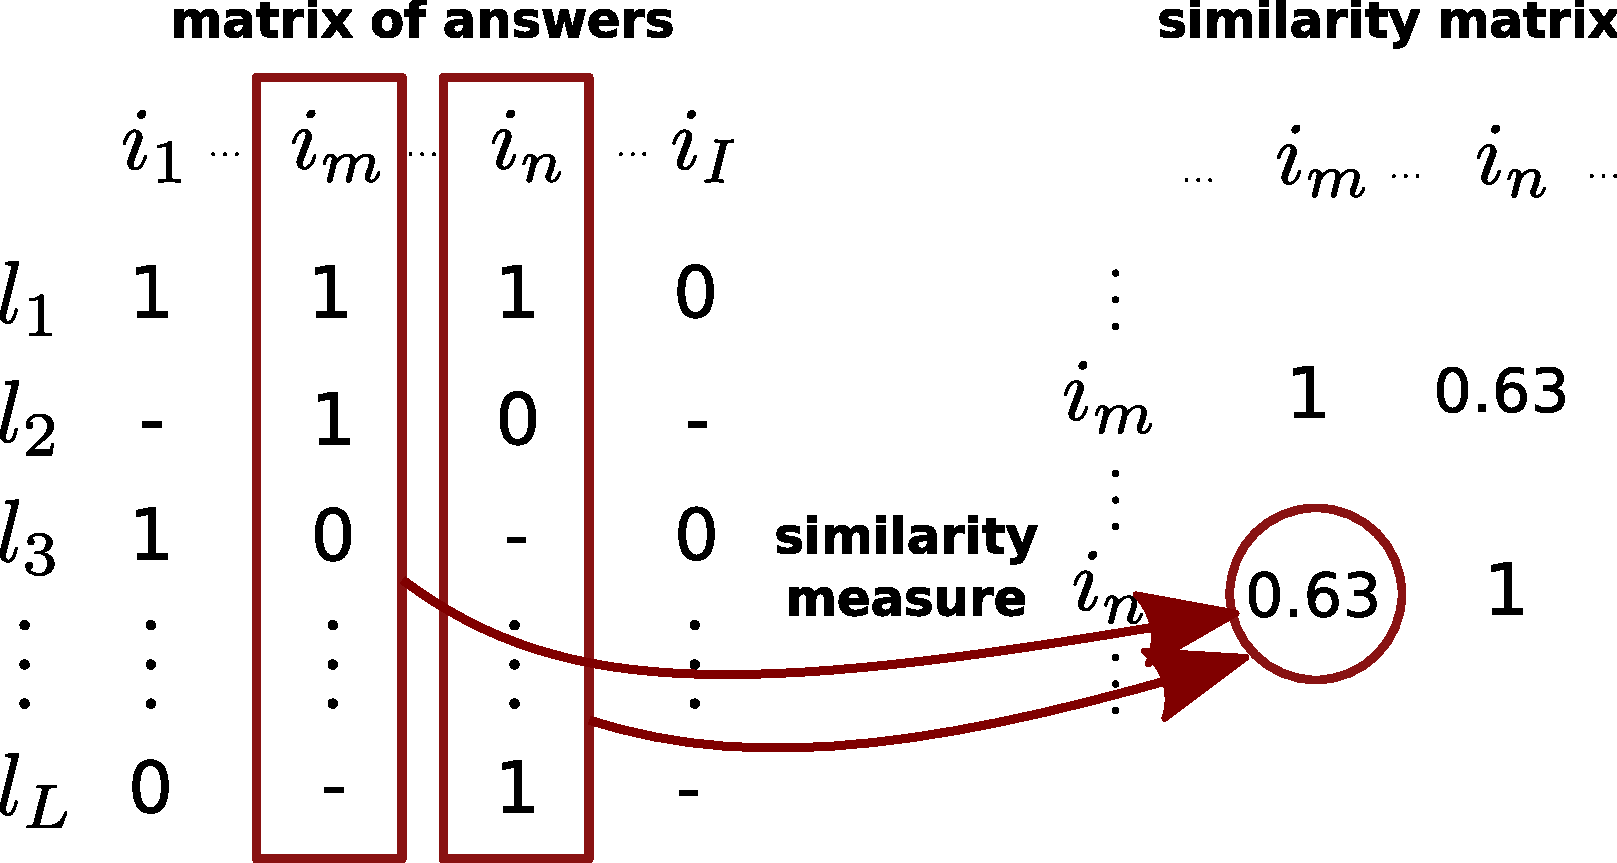
\includegraphics[width=.9\linewidth]{figures/diagram-first-step}
\end{frame}
% ------------------------------------------------------------------------------
% --------------------------- SLIDE --------------------------------------------
\begin{frame}
    \frametitle{Similarity measures}

    binary data
    \begin{itemize}
        \item $1$ --- correct
        \item $0$ --- incorrect
        \item input can be simplified:
    \end{itemize}

    \vfill

    \centering
    \begin{tabular}{llll}
        \toprule
        & & \multicolumn{2}{c}{item $i$} \\
        & & incorrect & correct \\
        \midrule
        item $j$ & incorrect & $a$ & $b$ \\
        & correct & $c$ & $d$ \\
        \bottomrule
    \end{tabular}
\end{frame}
% ------------------------------------------------------------------------------% --------------------------- SLIDE --------------------------------------------
\begin{frame}
    \frametitle{Similarity measures}

    \begin{center}
        \begin{tabular}{ll}
             Yule & $S_y = (ad-bc) / (ad+bc)$ \\[2mm]
             Pearson  &   $S_p = (ad - bc) /
             \sqrt{(a+b)(a+c)(b+d)(c+d)}$ \\[2mm]
             Cohen &   $S_c = (P_o - P_e) / (1 - P_e)$ \\
             & $ P_o = (a + d) / n$ \\
             & $P_e = ((a+b)(a+c) + (b+d)(c+d)) / n^2$\\[2mm]
             Sokal & $S_s = (a+d) / (a+b+c+d)$ \\[2mm] % Sokal-Michener
             Jaccard & $S_j = a / (a+b+c)$ \\[2mm]
             Ochiai &  $S_o = a / \sqrt{(a+b)(a+c)}$ \\
        \end{tabular}
    \end{center}
\end{frame}
% ------------------------------------------------------------------------------
% --------------------------- SLIDE --------------------------------------------
\begin{frame}
    \frametitle{Second level of similarity}
    \centering
    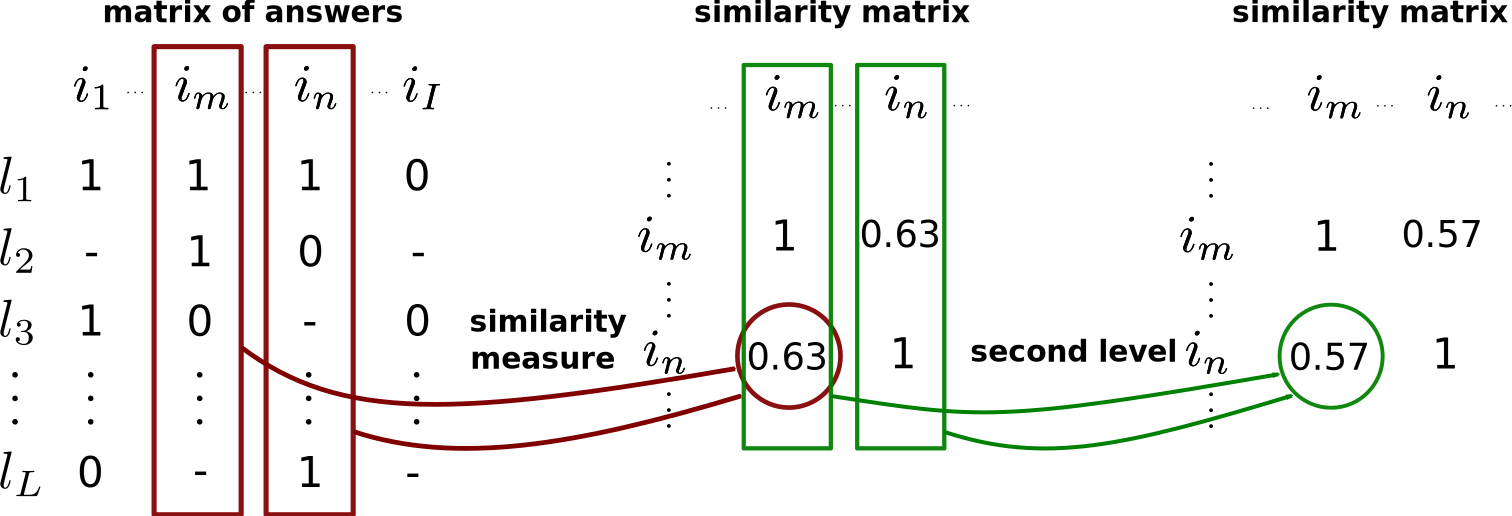
\includegraphics[width=\linewidth]{figures/diagram-second-step}
\end{frame}
% ------------------------------------------------------------------------------
% --------------------------- SLIDE --------------------------------------------
\begin{frame}
    \frametitle{Second level of similarity}
    \Large
    \begin{itemize}
        \item 2 items are similar if they are \emph{similarly} similar to other items
        \item more information used
        \item noise reduction
        \item necessary for some follow up algorithms
    \end{itemize}
\end{frame}
% ------------------------------------------------------------------------------
% --------------------------- SLIDE --------------------------------------------
\begin{frame}
    \frametitle{Evaluation - correlation of measures}
    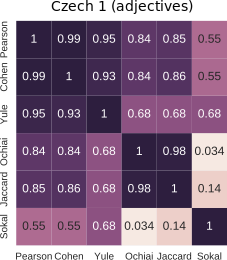
\includegraphics[width=\linewidth]{figures/measures-correlations}
\end{frame}
% ------------------------------------------------------------------------------
% --------------------------- SLIDE --------------------------------------------
\begin{frame}
    \frametitle{Evaluation - correlation of measures}
    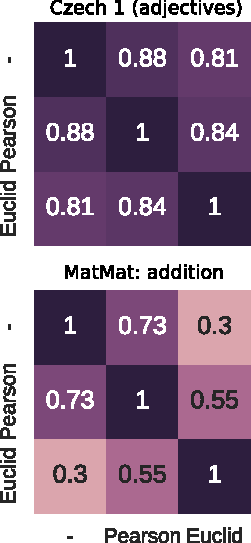
\includegraphics[width=\linewidth]{figures/measures-correlations2}
\end{frame}
% ------------------------------------------------------------------------------
% --------------------------- SLIDE --------------------------------------------
\begin{frame}
    \frametitle{Simulated data}
    \Large
    Simulated data
    \begin{itemize}
        \item we know \emph{right answer}
        \item logistic model
        \begin{itemize}
            \large
            \item learners have skills
            \item items have difficulty
        \end{itemize}
        \item typical setting
        \begin{itemize}
            \large
            \item $100$ learners
            \item $5$ knowledge components
            \item $20$ items per KC
        \end{itemize}
    \end{itemize}
\end{frame}
% ------------------------------------------------------------------------------
% --------------------------- SLIDE --------------------------------------------
\begin{frame}
    \frametitle{Evaluation}
    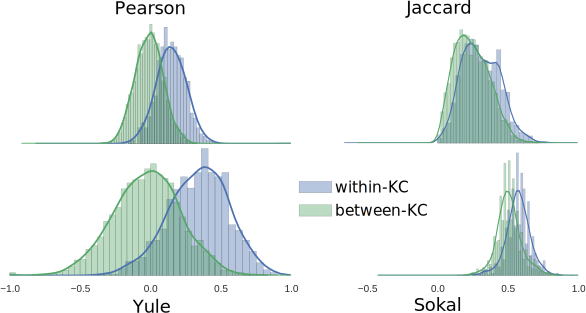
\includegraphics[width=\linewidth]{figures/measure-histograms}
\end{frame}
% ------------------------------------------------------------------------------
% --------------------------- SLIDE --------------------------------------------
\begin{frame}
    \frametitle{Evaluation}
    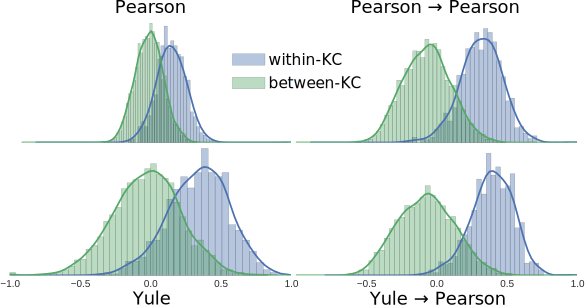
\includegraphics[width=\linewidth]{figures/measure-histograms2}
\end{frame}
% ------------------------------------------------------------------------------
% --------------------------- SLIDE --------------------------------------------
\begin{frame}
    \frametitle{Evaluation}
    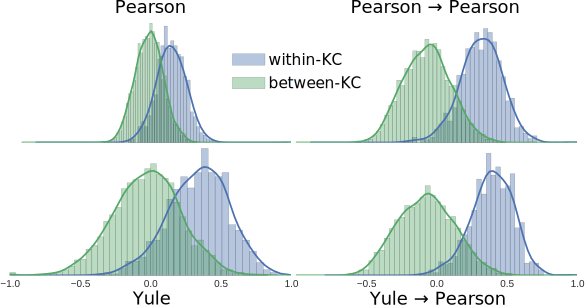
\includegraphics[width=\linewidth]{figures/measure-histograms2}
\end{frame}
% ------------------------------------------------------------------------------
% --------------------------- SLIDE --------------------------------------------
\begin{frame}
    \frametitle{Evaluation - clustering}
    \begin{tabular}{lcccccc}
        \toprule
                                   & Czech adjectives           &  100L 5KC             & 200L 5KC             \\
        \midrule

        Pearson                       & $        0.32 \pm 0.02$ &  $        0.48 \pm 0.05$ & $        0.84 \pm 0.05$ \\
        Jaccard                       & $        0.31 \pm 0.03$ &  $        0.15 \pm 0.04$ & $        0.29 \pm 0.08$ \\
        Yule                          & $        0.31 \pm 0.03$ &  $        0.43 \pm 0.05$ & $        0.77 \pm 0.07$ \\
        Sokal                         & $        0.15 \pm 0.06$ &  $        0.18 \pm 0.03$ & $        0.25 \pm 0.05$ \\
        Pearson $\rightarrow$ Euclid  & $\textbf{0.43}\pm 0.01$ &  $\textbf{0.80}\pm 0.06$ & $\textbf{0.98}\pm 0.01$ \\
        Yule    $\rightarrow$ Euclid  & $        0.32 \pm 0.02$ &  $        0.65 \pm 0.07$ & $        0.94 \pm 0.04$ \\
        Pearson $\rightarrow$ Pearson & $        0.41 \pm 0.03$ &  $        0.73 \pm 0.06$ & $        0.96 \pm 0.02$ \\
        Yule    $\rightarrow$ Pearson & $        0.32 \pm 0.03$ &  $        0.72 \pm 0.06$ & $        0.97 \pm 0.02$ \\
      \bottomrule
    \end{tabular}
\end{frame}
% ------------------------------------------------------------------------------
% --------------------------- SLIDE --------------------------------------------
\begin{frame}
    \frametitle{Do We Have Enough Data?}
    \begin{itemize}
        \item stability of results
        \item split data to two halves
        \item how similarity measures correlate on these halves?
    \end{itemize}
\end{frame}
% ------------------------------------------------------------------------------
% --------------------------- SLIDE --------------------------------------------
\begin{frame}
    \frametitle{Do We Have Enough Data?}
    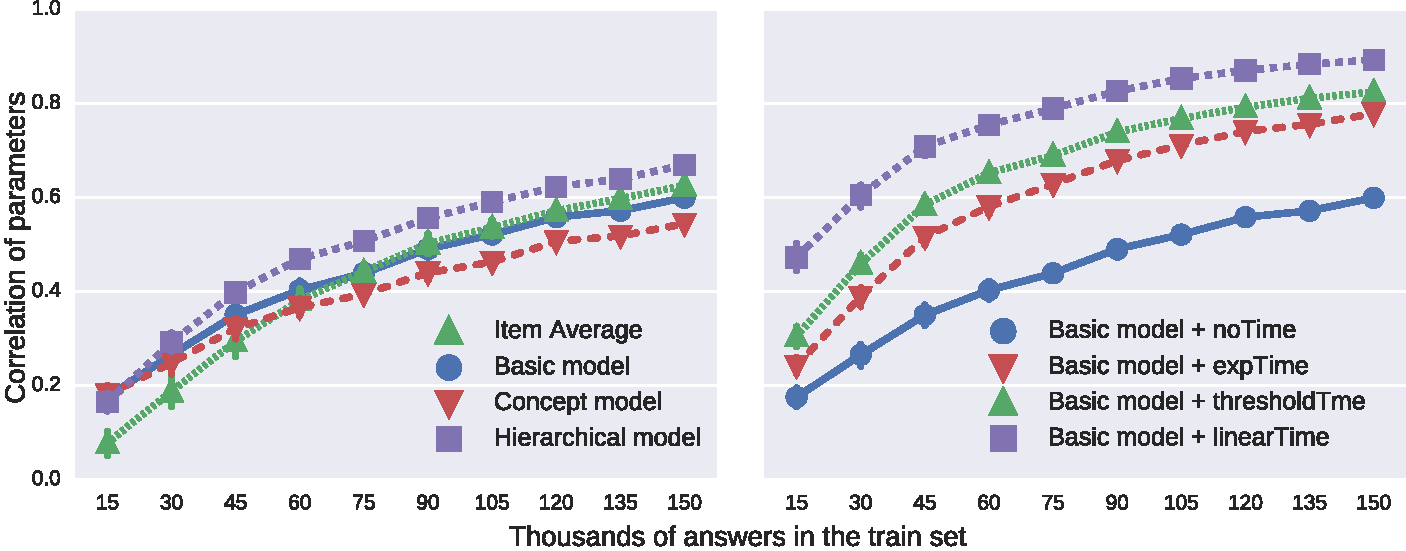
\includegraphics[width=\linewidth]{figures/stability}
\end{frame}
% ------------------------------------------------------------------------------
% --------------------------- SLIDE --------------------------------------------
\begin{frame}
    \frametitle{Response times}
    \begin{itemize}
        \item additional information
        \item correctness and response time to one measure of success
    \end{itemize}

    \vfill

    \centering
    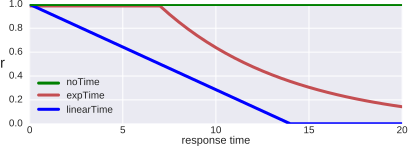
\includegraphics[width=0.8\linewidth]{figures/time-uses}

\end{frame}
% ------------------------------------------------------------------------------
% --------------------------- SLIDE --------------------------------------------
\begin{frame}
    \frametitle{Respose times - MathMat}
    \centering
    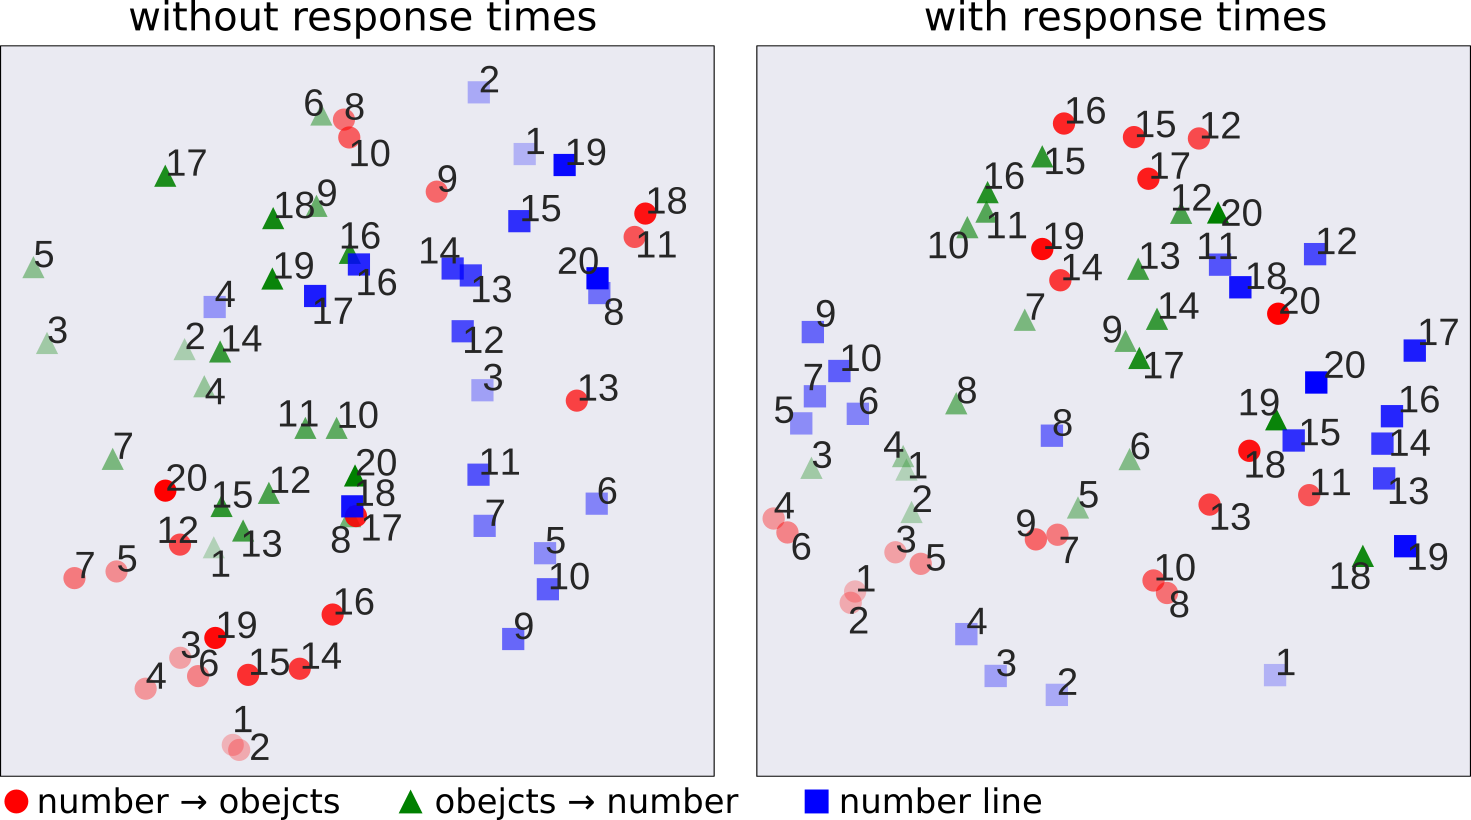
\includegraphics[width=\linewidth]{figures/matmat-projection-time}
\end{frame}
% ------------------------------------------------------------------------------
% --------------------------- SLIDE --------------------------------------------
\begin{frame}
    \frametitle{Respose times - Math Garden}
    \begin{itemize}
        \item Math Garden - large datasets: $\sim 1M$ of answer on $30$ items
        \item small impact of time information - correlation $>0.9$
        \item but what we have not such large dataset

    \end{itemize}
\end{frame}
% ------------------------------------------------------------------------------
% --------------------------- SLIDE --------------------------------------------
\begin{frame}
    \frametitle{Respose times - MathGarden}
    \centering
    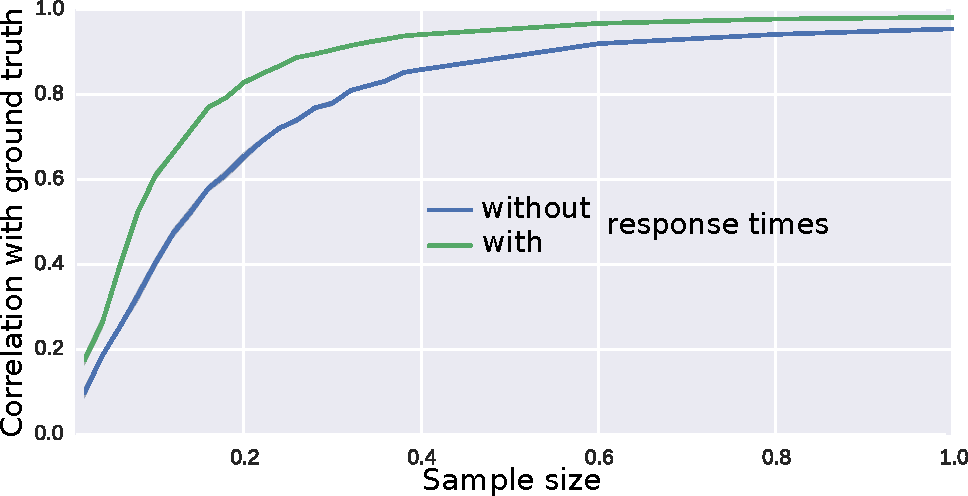
\includegraphics[width=\linewidth]{figures/measure-convergence-time}
\end{frame}
% ------------------------------------------------------------------------------
% --------------------------- SLIDE --------------------------------------------
\begin{frame}
    \frametitle{Conclusion}
    \Large
    \begin{itemize}
        \item Pearson (Cohen) and Yule are better
        \item second level improve results
        \item we should check that we have sufficient data
        \item response time can give different point of view
        \item response time can help with small datasets
    \end{itemize}
\end{frame}
% ------------------------------------------------------------------------------




\end{document}
% ------------------------------------------------------------------------------
% ------------------------------------------------------------------------------
% ------------------------------------------------------------------------------
% --------------------------- SLIDE --------------------------------------------
\begin{frame}
    \frametitle{}
\end{frame}
% ------------------------------------------------------------------------------
\begin{itemize}
\end{itemize}
